% Drawing 146/04-14 -- folder 146, batch 04, archive page 76 (PDF page 77).
% Transcription: Feuillet en largeur, presque entièrement de figures : trois sphères à gauche, dont l'équateur porte des points cerclés étiquetés $a, b, c, d, e$ et $s, t, u, v, w$, avec un pôle $a$ relié par des méridiens, un secteur hachuré et des flèches de rotation ; au centre, un grand patron (un pentagone en perspective, sommets $s$, $t$, et des faces hachurées) dont les arêtes portent $(a), (b), (c), (d), (e)$ ; au-dessous, une sphère et deux cercles équatoriaux portant les mêmes lettres ; en haut à droite, un fuseau de sommets $s$ et $t$, arêtes $b, c, d, e$, une région hachurée et un point $\alpha$.
% Kind: page of figures (spheres with ringed points, a net, a lune). Method 2 (schematic redraw from the facsimile). Status: ok.
% Notes: Landscape sheet, redrawn figure by figure on tight crops. On every sphere and circle the ringed points are placed on the equator ellipse (projected) and each meridian ends at a ringed point or a pole. Left column: sphere 1 (ringed c, b, a, d, e and the small ring by s on the equator, letters u-w, s, t; the hatched wedge from one point to a; rotation arrow); sphere 2 (top point a joined to the four ringed points, the two back meridians dotted, hatched sector, rotation arrow, the inked point at the right end of the equator); sphere 3 (pole a, back meridians dashed, the bold front meridian through e to the bottom, hatched sector). The net: the pentagon s-t-u-v-w in perspective as one curve through its five vertices and the five ringed points d, c, b, a, e on its sides; the inner point joined to u and s and (dashed) to t and w; the hatched triangle; the faces round it, every stroke between named vertices: quadrilateral (b) on the left, triangle (a)/(e), the central stroke (c) from s to the fork with (d) and (b), the strokes (d), (e) on the right from t, the small triangle with the arrow and (b) and the dashed strokes (e). Bottom: the sphere with pole a, ringed c, b, d, e, s, alpha, the rotation arrow; the circle c, b, d, e with the two strokes down to a ring; the circle c, b, a, d with the heavy ring and the arrow up. Top right: the lune s-t with c, d, b, e, the chord through alpha (dashed beyond), the hatched region. Left out: the scribbled (struck) region over the left triangle of the net, labelled « (c) »/« (e) »; the text at the right (R, repères ...). Still differs: the faces of the net are a reading of faint pencil, not encoded; letter positions approximate; his doubled outlines are drawn once. Redrawn 2026-11-09 (issue 128): to check again.
% Coordinates: 1 unit = 1 mm = 1/100 of the crop width (bbox in page fractions: [0.13, 0.095, 0.8, 0.41]).
% Redrawn by Claude (claude-opus-5-5), issue #73, 2026-11-09; not checked by a human; not compiled (no TeX in the session).
% Rights: reproduces part of the work -- behind RENDER_TRANSCRIPTS, never published by itself.
% Revised by Claude (claude-sonnet-5-5) 2026-11-11 after Michel's check (#142): confirmed as redrawn. Status: ok.
\documentclass[tikz,border=3pt]{standalone}
\usepackage{amsmath,amssymb}
\usetikzlibrary{patterns,arrows.meta}
\tikzset{pencil/.style={black!45}, struck/.style={black!35}, mark/.style={circle,draw,inner sep=1.3pt}, pt/.style={circle,fill,inner sep=0.9pt}, opt/.style={circle,draw,fill=white,inner sep=1.1pt}}
\begin{document}
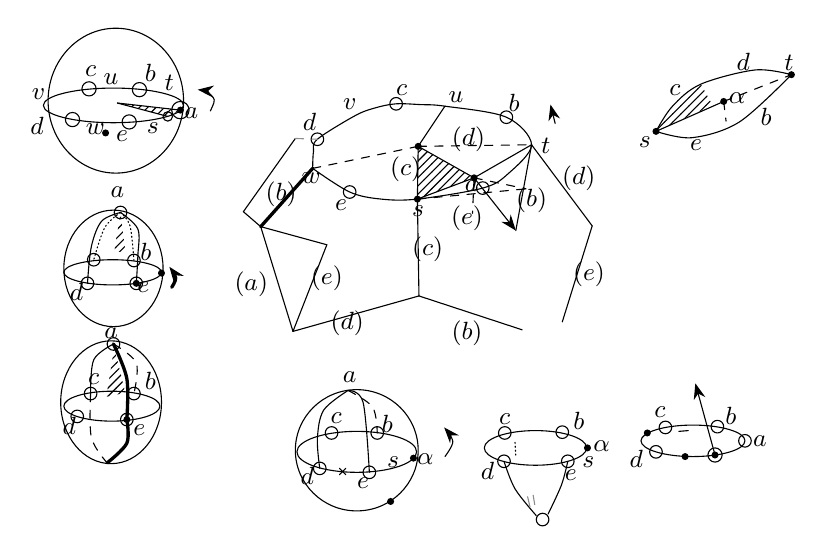
\begin{tikzpicture}[x=1mm,y=1mm,line cap=round,line join=round,font=\scriptsize]
\draw (13.8,-10.7) ellipse[x radius=8.6, y radius=9.2];
\draw (13.5,-11.3) ellipse[x radius=8.9, y radius=2.2];
\draw (10.4,-9.2) circle[radius=0.9];
\draw (16.8,-9.3) circle[radius=0.9];
\draw (22,-11.9) circle[radius=1.1];
\node[pt] at (22,-11.9) {};
\draw (8.3,-13.1) circle[radius=0.9];
\draw (15.5,-13.4) circle[radius=0.9];
\draw (20.4,-12.7) circle[radius=0.6];
\draw (14,-11) -- (22,-11.9);
\draw (14,-11) -- (20.4,-12.7);
\fill[pattern=north east lines] (14,-11) -- (22,-11.9) -- (20.4,-12.7) -- cycle;
\node[pt] at (12.5,-14.8) {};
\draw[-{Stealth[length=2mm]}] plot[smooth, tension=0.55] coordinates {(25.8,-12) (26.3,-10.6) (25.4,-9.6) (24.2,-9.3)};
\node[inner sep=1pt] at (4,-9.9) {\small $v$};
\node[inner sep=1pt] at (10.6,-6.9) {\small $c$};
\node[inner sep=1pt] at (13.2,-8) {\small $u$};
\node[inner sep=1pt] at (18.2,-7.2) {\small $b$};
\node[inner sep=1pt] at (20.6,-8.4) {\small $t$};
\node[inner sep=1pt] at (23.4,-12.3) {\small $a$};
\node[inner sep=1pt] at (3.8,-13.9) {\small $d$};
\node[inner sep=1pt] at (11.2,-14.3) {\small $w$};
\node[inner sep=1pt] at (14.6,-15.2) {\small $e$};
\node[inner sep=1pt] at (18.5,-14.2) {\small $s$};
\draw (13.5,-32) ellipse[x radius=6.3, y radius=7.4];
\draw (13.4,-32.5) ellipse[x radius=6.2, y radius=1.6];
\draw plot[smooth, tension=0.55] coordinates {(14.4,-24.9) (12,-26) (10.7,-29.2) (10.2,-33.9)};
\draw[densely dotted] plot[smooth, tension=0.55] coordinates {(14.4,-24.9) (12.4,-26.8) (11,-30.9)};
\draw[densely dotted] plot[smooth, tension=0.55] coordinates {(14.4,-24.9) (15.6,-26.6) (16.1,-31)};
\draw plot[smooth, tension=0.55] coordinates {(14.4,-24.9) (16.6,-27) (16.6,-30.4) (16.4,-33.9)};
\fill[pattern=north east lines] (14.4,-24.9) -- (13.6,-29.9) -- (15,-29.9) -- cycle;
\draw (14.4,-24.9) circle[radius=0.8];
\draw (11,-30.9) circle[radius=0.8];
\draw (16.1,-31) circle[radius=0.8];
\draw (10.2,-33.9) circle[radius=0.8];
\draw (16.4,-33.9) circle[radius=0.8];
\node[pt] at (16.4,-33.9) {};
\node[pt] at (19.6,-32.6) {};
\draw[very thick,-{Stealth[length=2mm]}] plot[smooth, tension=0.55] coordinates {(20.9,-34.4) (21.4,-33.2) (20.6,-31.8)};
\node[inner sep=1pt] at (14,-22.3) {\small $a$};
\node[inner sep=1pt] at (17.6,-29.9) {\small $b$};
\node[inner sep=1pt] at (8.8,-35) {\small $d$};
\node[inner sep=1pt] at (17.3,-34.4) {\small $e$};
\draw (13.2,-49) ellipse[x radius=6.4, y radius=7.8];
\draw (13.3,-49.5) ellipse[x radius=6.1, y radius=1.9];
\draw plot[smooth, tension=0.55] coordinates {(13.5,-41.6) (11,-43.6) (10.6,-47.9)};
\draw[dashed] plot[smooth, tension=0.55] coordinates {(10.6,-47.9) (10.7,-53.5) (12.7,-56.7)};
\draw[dashed] plot[smooth, tension=0.55] coordinates {(13.5,-41.6) (16.4,-44) (16.1,-47.9)};
\draw[very thick] plot[smooth, tension=0.55] coordinates {(13.5,-41.6) (15.2,-46) (15.2,-51.2)};
\draw[very thick] plot[smooth, tension=0.55] coordinates {(15.2,-51.2) (15.2,-54.2) (12.7,-56.7)};
\fill[pattern=north east lines] (13.6,-42) -- (12.6,-48.3) -- (15,-47.8) -- cycle;
\draw (13.5,-41.6) circle[radius=0.8];
\draw (10.6,-47.9) circle[radius=0.8];
\draw (16.1,-47.9) circle[radius=0.8];
\draw (8.9,-50.8) circle[radius=0.8];
\draw (15.2,-51.2) circle[radius=0.8];
\node[pt] at (15.2,-51.2) {};
\node[inner sep=1pt] at (13.2,-40.2) {\small $a$};
\node[inner sep=1pt] at (11,-46.1) {\small $c$};
\node[inner sep=1pt] at (18.2,-46.3) {\small $b$};
\node[inner sep=1pt] at (7.9,-52) {\small $d$};
\node[inner sep=1pt] at (16.8,-52.6) {\small $e$};
\draw plot[smooth, tension=0.55] coordinates {(38.8,-19.3) (38.9,-17.2) (39.4,-15.6) (44.2,-12.6) (46.8,-11.6) (49.4,-11.1) (52.5,-11.2) (55.6,-11.4) (63.4,-12.8) (66.6,-16.3) (63.6,-20) (60.4,-21.8) (52.1,-23.2) (47.5,-23.2) (43.5,-22.3) (38.8,-19.3)};
\draw (39.4,-15.6) circle[radius=0.8];
\draw (49.4,-11.1) circle[radius=0.8];
\draw (63.4,-12.8) circle[radius=0.8];
\draw (60.4,-21.8) circle[radius=0.8];
\draw (43.5,-22.3) circle[radius=0.8];
\draw (52.2,-16.5) -- (55.6,-11.4);
\draw (52.2,-16.5) -- (52.1,-23.2);
\draw (52.2,-16.5) -- (59.3,-20.5);
\draw (66.6,-16.3) -- (59.3,-20.5);
\draw (59.3,-20.5) -- (52.1,-23.2);
\draw (66.6,-16.3) -- (64.6,-27.2);
\draw (36.6,-15.5) -- (30,-24.8);
\draw (30,-24.8) -- (32.2,-26.7);
\draw (32.2,-26.7) -- (40.6,-29);
\draw (32.2,-26.7) -- (36.3,-40);
\draw (40.6,-29) -- (36.3,-40);
\draw (36.3,-40) -- (52.3,-35.5);
\draw (52.1,-23.2) -- (52.3,-35.5);
\draw (52.3,-35.5) -- (65.4,-39.8);
\draw (66.6,-16.3) -- (74.3,-26.6);
\draw (74.3,-26.6) -- (70.5,-38.8);
\draw[-{Stealth[length=2mm]}] (59.3,-20.5) -- (64.6,-27.2);
\draw[very thick] (32.2,-26.7) -- (38.8,-19.3);
\draw[dashed] (52.2,-16.5) -- (66.6,-16.3);
\draw[dashed] (52.2,-16.5) -- (38.8,-19.3);
\draw[dashed] (59.3,-20.5) -- (65.9,-21.9);
\draw[dashed] (52.1,-23.2) -- (65.9,-21.9);
\draw[dashed] (59.3,-20.5) -- (59.1,-25);
\draw[dashed,pencil] (36.6,-15.5) -- (39.4,-15.6);
\fill[pattern=north east lines] (52.2,-16.5) -- (52.1,-23.2) -- (59.3,-20.5) -- cycle;
\node[pt] at (52.2,-16.5) {};
\node[pt] at (52.1,-23.2) {};
\node[pt] at (59.3,-20.5) {};
\draw[-{Stealth[length=2mm]}] (69.6,-13.6) -- (69,-11.2);
\node[inner sep=1pt] at (38.4,-13.4) {\small $d$};
\node[inner sep=1pt] at (43.5,-11.2) {\small $v$};
\node[inner sep=1pt] at (50.1,-9.3) {\small $c$};
\node[inner sep=1pt] at (57,-10.3) {\small $u$};
\node[inner sep=1pt] at (64.4,-11) {\small $b$};
\node[inner sep=1pt] at (68.4,-16.4) {\small $t$};
\node[inner sep=1pt] at (58.6,-15.6) {\small $(d)$};
\node[inner sep=1pt] at (50.6,-19.4) {\small $(c)$};
\node[inner sep=1pt] at (59,-21.6) {\small $a$};
\node[inner sep=1pt] at (38.6,-20.6) {\small $w$};
\node[inner sep=1pt] at (42.4,-24) {\small $e$};
\node[inner sep=1pt] at (52.2,-24.7) {\small $s$};
\node[inner sep=1pt] at (58.4,-25.6) {\small $(e)$};
\node[inner sep=1pt] at (66.6,-23.4) {\small $(b)$};
\node[inner sep=1pt] at (72.6,-20.6) {\small $(d)$};
\node[inner sep=1pt] at (34.8,-22.6) {\small $(b)$};
\node[inner sep=1pt] at (31,-34) {\small $(a)$};
\node[inner sep=1pt] at (40.6,-33.2) {\small $(e)$};
\node[inner sep=1pt] at (53.4,-29.6) {\small $(c)$};
\node[inner sep=1pt] at (73.9,-32.8) {\small $(e)$};
\node[inner sep=1pt] at (43.2,-39) {\small $(d)$};
\node[inner sep=1pt] at (58.4,-40.2) {\small $(b)$};
\draw (44.4,-55.1) ellipse[x radius=7.8, y radius=7.7];
\draw (44.4,-55.3) ellipse[x radius=7.6, y radius=2.6];
\draw plot[smooth, tension=0.55] coordinates {(43.3,-47.5) (40.2,-50) (39.4,-53.6) (39.7,-57.4)};
\draw plot[smooth, tension=0.55] coordinates {(43.3,-47.5) (45.2,-49) (46,-57.9)};
\draw[dashed] plot[smooth, tension=0.55] coordinates {(43.3,-47.5) (46.4,-49.6) (47,-52.9)};
\draw (41.2,-52.9) circle[radius=0.8];
\draw (47,-52.9) circle[radius=0.8];
\draw (39.7,-57.4) circle[radius=0.8];
\draw (46,-57.9) circle[radius=0.8];
\node[pt] at (51.6,-56.1) {};
\node[pt] at (48.7,-61.6) {};
\draw (42.2,-57.4) -- (43,-58.2);
\draw (42.2,-58.2) -- (43,-57.4);
\draw[-{Stealth[length=2mm]}] plot[smooth, tension=0.55] coordinates {(55.6,-55.9) (56.6,-54) (55.5,-52.2)};
\node[inner sep=1pt] at (43.5,-45.8) {\small $a$};
\node[inner sep=1pt] at (41.8,-51) {\small $c$};
\node[inner sep=1pt] at (48.3,-51.8) {\small $b$};
\node[inner sep=1pt] at (38.1,-58.4) {\small $d$};
\node[inner sep=1pt] at (45.2,-59.3) {\small $e$};
\node[inner sep=1pt] at (49,-56.6) {\small $s$};
\node[inner sep=1pt] at (53.1,-56.2) {\small $\alpha$};
\draw (67.1,-54.8) ellipse[x radius=6.5, y radius=2.2];
\draw (63.2,-52.9) circle[radius=0.8];
\draw (70.5,-52.8) circle[radius=0.8];
\draw (63.1,-56.5) circle[radius=0.8];
\draw (71.2,-56.5) circle[radius=0.8];
\node[pt] at (73.7,-54.8) {};
\draw plot[smooth, tension=0.55] coordinates {(63.1,-56.5) (64.5,-60) (67.2,-63.4)};
\draw plot[smooth, tension=0.55] coordinates {(71.2,-56.5) (70.4,-59.5) (68.7,-63.2)};
\draw (68,-63.9) circle[radius=0.8];
\draw[densely dotted] (64.5,-54.1) -- (64.6,-55.9);
\draw[pencil] (66.1,-61) -- (66.4,-62.3);
\draw[pencil] (66.8,-60.8) -- (67,-62);
\node[inner sep=1pt] at (63.2,-51.2) {\small $c$};
\node[inner sep=1pt] at (72.6,-51.4) {\small $b$};
\node[inner sep=1pt] at (75.5,-54.6) {\small $\alpha$};
\node[inner sep=1pt] at (61,-57.7) {\small $d$};
\node[inner sep=1pt] at (71.6,-58.2) {\small $e$};
\node[inner sep=1pt] at (73.8,-56.6) {\small $s$};
\draw (87.1,-53.9) ellipse[x radius=6.6, y radius=2];
\draw (83.6,-52.2) circle[radius=0.8];
\draw (90.2,-52.1) circle[radius=0.8];
\draw (93.7,-53.9) circle[radius=0.8];
\draw (82.4,-55.3) circle[radius=0.8];
\draw (89.9,-55.7) circle[radius=0.9];
\node[pt] at (89.9,-55.7) {};
\draw[-{Stealth[length=2mm]}] (89.9,-55.7) -- (87.4,-46.6);
\draw (85.3,-52.7) -- (86.5,-52.6);
\node[pt] at (81.3,-52.9) {};
\node[pt] at (86.1,-55.9) {};
\node[inner sep=1pt] at (82.9,-50.2) {\small $c$};
\node[inner sep=1pt] at (91.9,-50.7) {\small $b$};
\node[inner sep=1pt] at (95.6,-54) {\small $a$};
\node[inner sep=1pt] at (79.9,-56.2) {\small $d$};
\draw plot[smooth, tension=0.55] coordinates {(82.4,-14.6) (84.5,-11.4) (88.1,-8.6) (95,-6.8) (99.6,-7.4)};
\draw plot[smooth, tension=0.55] coordinates {(82.4,-14.6) (87,-15.4) (93,-13.4) (99.6,-7.4)};
\draw (82.4,-14.6) -- (91,-10.8);
\draw[dashed] (91,-10.8) -- (99.6,-7.4);
\draw[dashed] (91,-10.8) -- (91.3,-13.3);
\fill[pattern=north east lines] (82.4,-14.6) -- (84.5,-11.4) -- (88.1,-8.6) -- (89.6,-11.3) -- cycle;
\node[pt] at (91,-10.8) {};
\node[pt] at (82.4,-14.6) {};
\node[pt] at (99.6,-7.4) {};
\node[inner sep=1pt] at (81,-16) {\small $s$};
\node[inner sep=1pt] at (99.3,-5.9) {\small $t$};
\node[inner sep=1pt] at (84.8,-9.3) {\small $c$};
\node[inner sep=1pt] at (93.5,-5.8) {\small $d$};
\node[inner sep=1pt] at (96.4,-12.7) {\small $b$};
\node[inner sep=1pt] at (87.5,-16.3) {\small $e$};
\node[inner sep=1pt] at (92.7,-10.4) {\small $\alpha$};
\end{tikzpicture}
\end{document}
